\section{MGK7MB - ICE Motherboard}
\label{sec_motherboard}

\begin{figure}[h]
	\centering
	\includegraphics[width=\linewidth]{./IceBoardPhotos/main_view.jpg}
	\caption{Motherboard}
	\label{fig:motherboard}
\end{figure}

\pagebreak
\subsection{Inspection Test}

\noindent \textbf{Step 1}: Is the FPGA heatsink securely attached?
\\*\textbf{Step 2}: Are the FPGA heatsink pins cut near the stiffener?
\begin{figure}[!htbp]
	\centering
	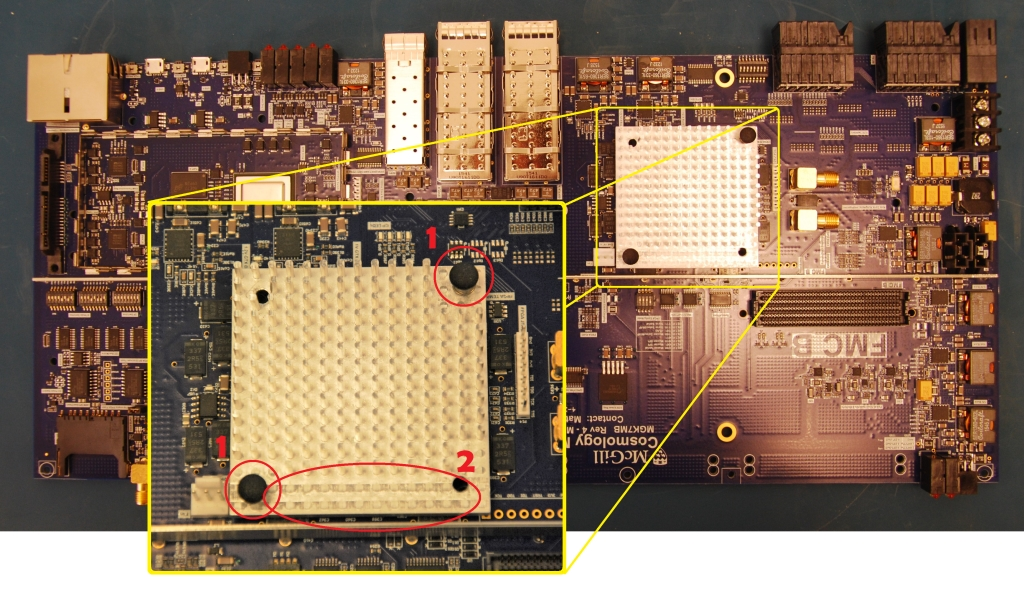
\includegraphics[width=\linewidth]{./IceBoardPhotos/InspTest/inspection_step12.jpeg}
	\caption{Points of interest for Steps 1 and 2}
	\label{fig:InspSteps1and2}
\end{figure}

\pagebreak
\noindent \textbf{Step 3}: Is the board stiffener installed, and the board reasonably flat?
\\*\textbf{Step 4}: Are the PLL heatsinks attached?
\\*\textbf{Step 5}: Does the arm shield fence look straight?
\begin{figure}[!htbp]
	\centering
	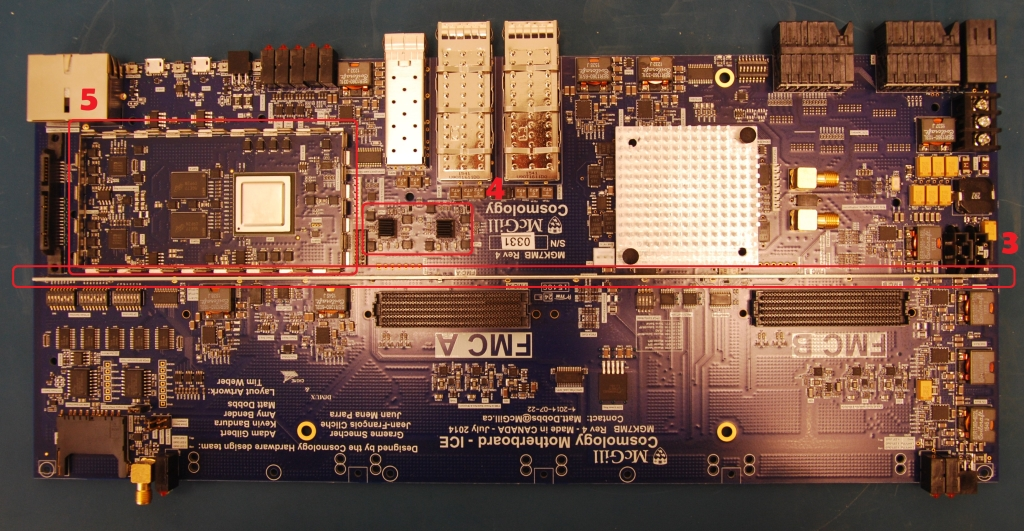
\includegraphics[width=\linewidth]{./IceBoardPhotos/InspTest/inspection_step345.jpeg}
	\caption{Points of interest for Steps 3,4 and 5}
	\label{fig:InspSteps34and5}
\end{figure}

\pagebreak
\noindent \textbf{Step 6}: Are the dipswitches set correctly?
\\*\textbf{Step 7}: Are the jumpers set correctly?
\begin{figure}[!htbp]
	\centering
	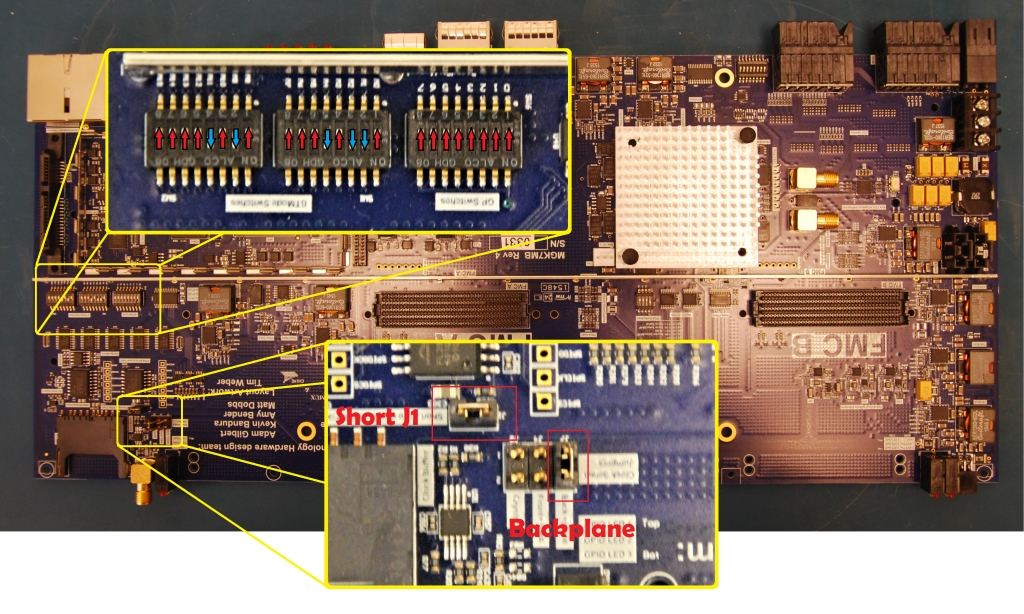
\includegraphics[width=\linewidth]{./IceBoardPhotos/InspTest/inspection_step67.jpeg}
	\caption{Points of interest for Steps 6 and 7}
	\label{fig:InspSteps6and7}
\end{figure}

\pagebreak
\noindent \textbf{Step 8}: Are the 90 pin Molex backplane connectors screwed down? (backside)
\\*\textbf{Step 9}: Are the QSFP and SFP connectors soldered in place? (backside)
\\*\textbf{Step 10}: Do all the buck converters have the additional hand-soldered capacitor? (backside)
\begin{figure}[!htbp]
	\centering
	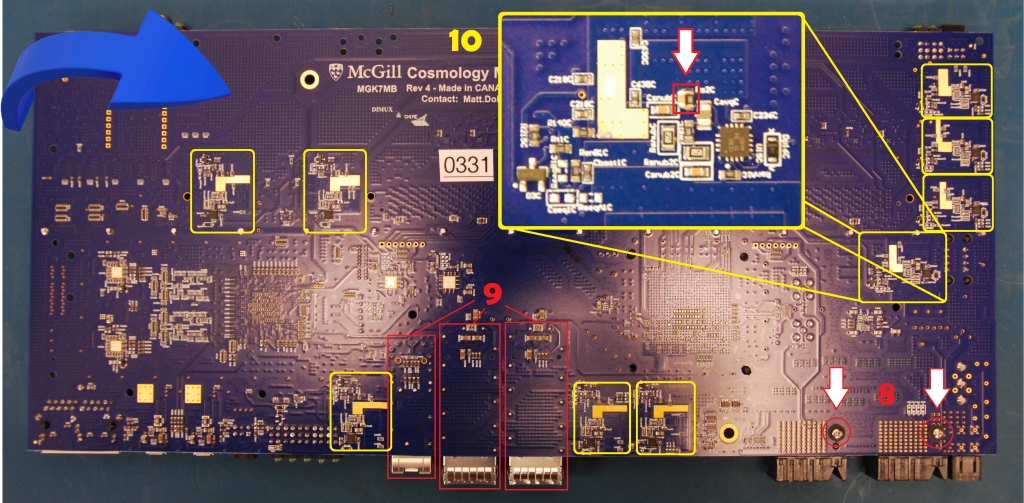
\includegraphics[width=\linewidth]{./IceBoardPhotos/InspTest/inspection_step8910.jpeg}
	\caption{Points of interest for Steps 8,9 and 10}
	\label{fig:InspSteps89and10}
\end{figure}

\pagebreak
\noindent \textbf{Step 11}: Do all the FMC power switches look well soldered?
\\*\textbf{Step 12}: Is the blue patch wire in place and secured?
\begin{figure}[!htbp]
	\centering
	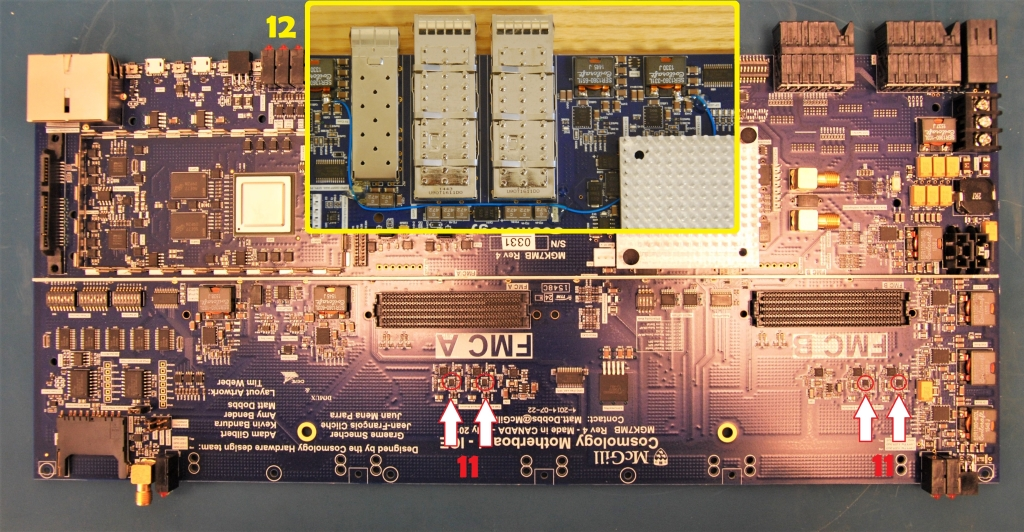
\includegraphics[width=\linewidth]{./IceBoardPhotos/InspTest/inspection_step1112.jpeg}
	\caption{Points of interest for Steps 11 and 12}
	\label{fig:InspSteps11and12}
\end{figure}

\pagebreak
\subsection{Impedance Test}
Before taking measurements, make sure that the board setup is as shown in figure \ref{fig:ImpSetup}.
\begin{figure}[!htbp]
	\centering
	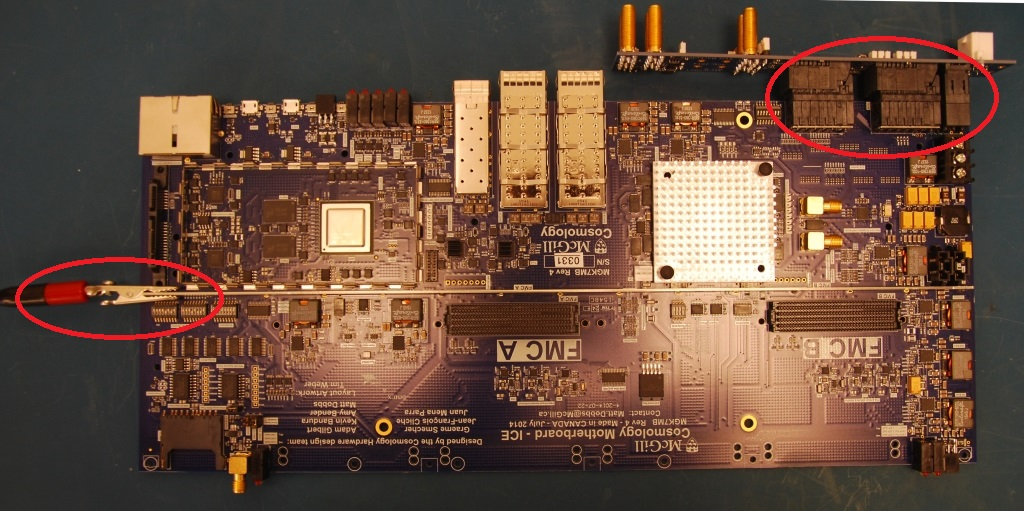
\includegraphics[width=\linewidth]{./IceBoardPhotos/ImpTest/CroppedIceboard.jpeg}
	\caption{Iceboard with ground connection and one-slot backplane }
	\label{fig:ImpSetup}
\end{figure}

Apply the red test probe to the test points in the following order: +V supply followed by the buck converters in a counter clockwise order - see figure \ref{fig:ImpLocs}. Refer to probe location 10 in the diagram for instructions on where to apply the test probe for all buck converters.

\begin{figure}[!htbp]
	\centering
	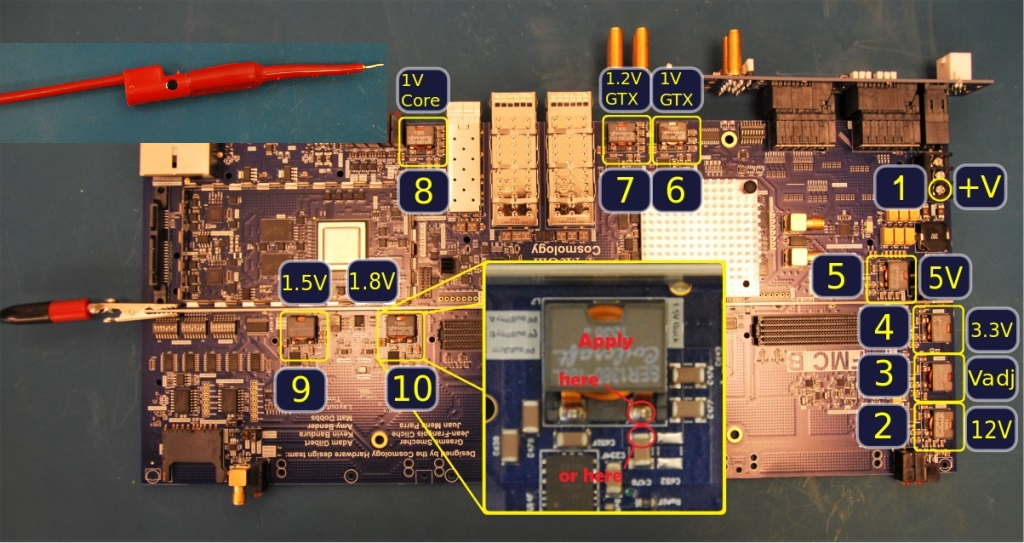
\includegraphics[width=\linewidth]{./IceBoardPhotos/ImpTest/Impedance_test-points.jpeg}
	\caption{Impedance measurement test locations }
	\label{fig:ImpLocs}
\end{figure}

\pagebreak
\subsection{Power Test}
Connect the power cable to the backplane as shown in figure \ref{fig:PowSetup}.

\begin{figure}[!htbp]
	\centering
	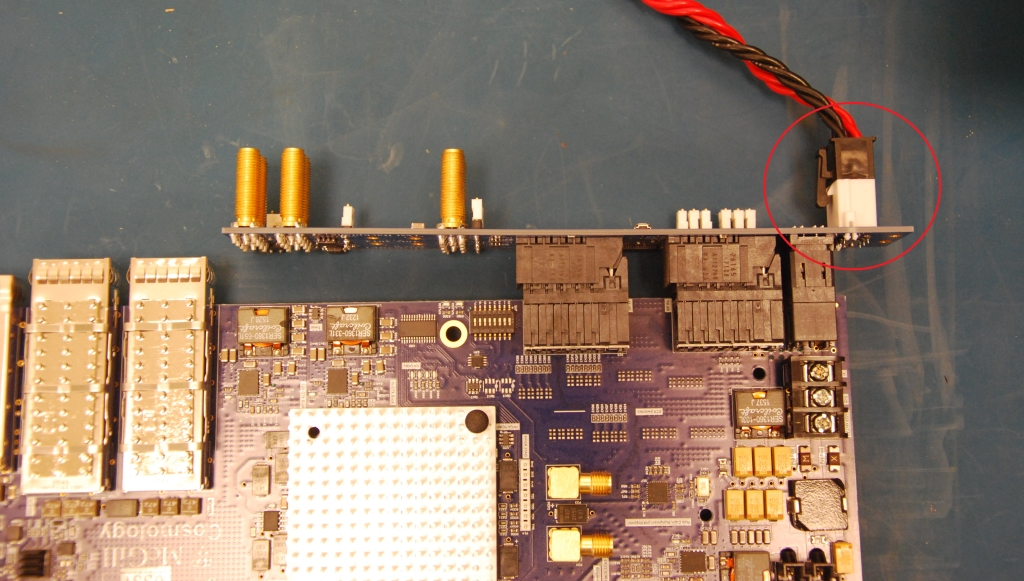
\includegraphics[width=\linewidth]{./IceBoardPhotos/PowerUpTest/power_cable.jpeg}
	\caption{Power cable attached to one-slot backplane with motherboard}
	\label{fig:PowSetup}
\end{figure}

Check that all 9 power LEDs are turned on as shown in figure \ref{fig:PowLEDs}.
\begin{figure}[!htbp]
	\centering
	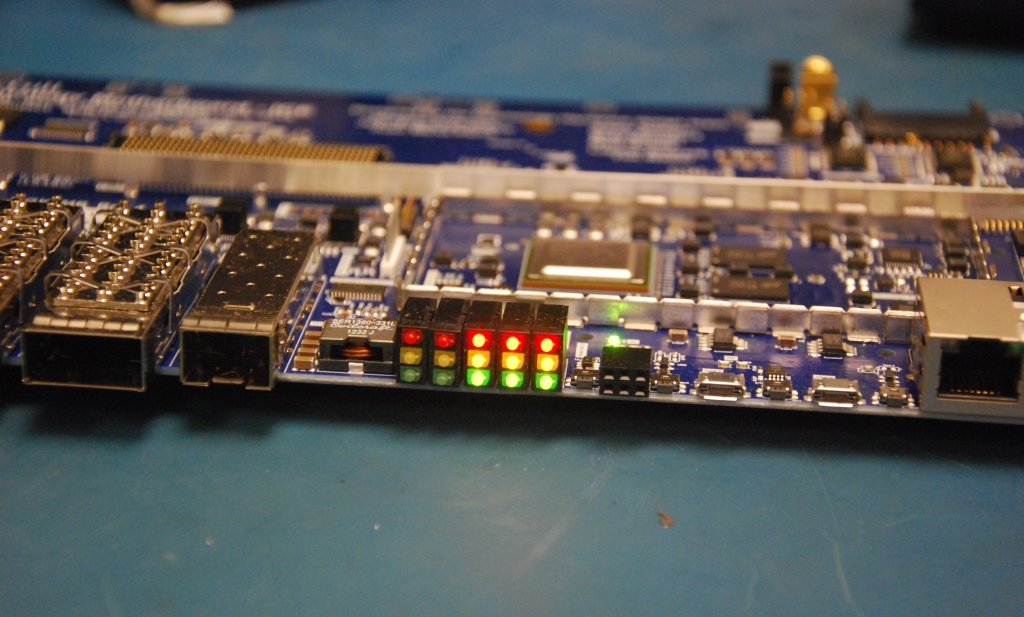
\includegraphics[width=\linewidth]{./IceBoardPhotos/PowerUpTest/power_leds.jpeg}
	\caption{Motherboards 9 power LEDS}
	\label{fig:PowLEDs}
\end{figure}

\pagebreak
\subsection{PLL Programming}
Connect the PLL programming cable to the board, making sure that the black marked side faces the SFP connectors - see figure \ref{fig:PLLDong}.

\begin{figure}[!htbp]
	\centering
	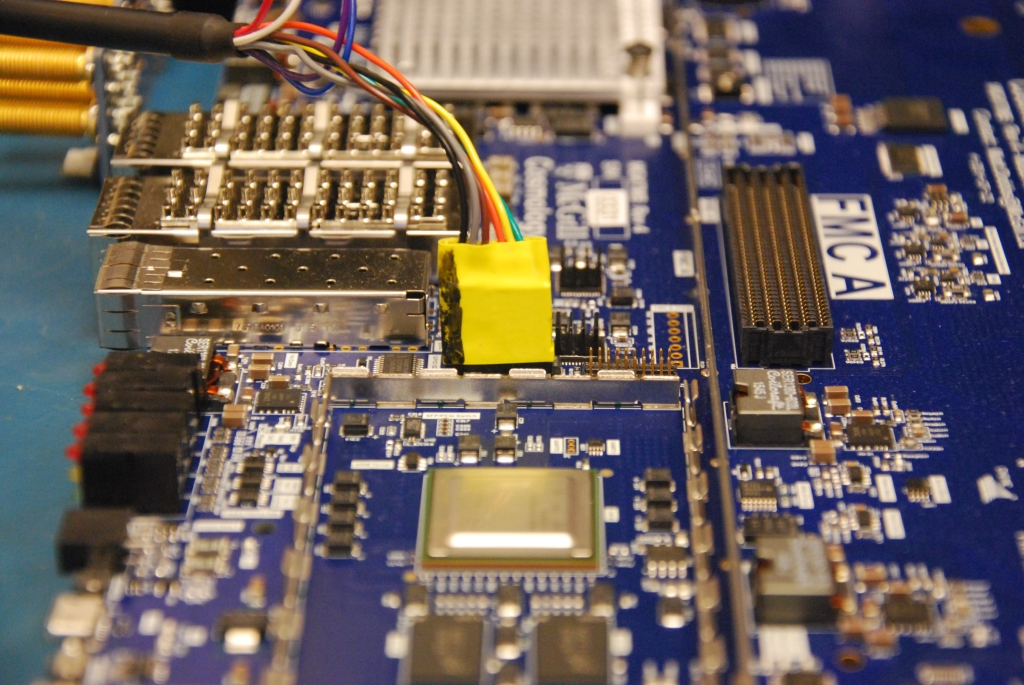
\includegraphics[width=0.7\linewidth]{./IceBoardPhotos/PLLTest/PLLDongle.jpeg}
	\caption{PLL Programming dongle}
	\label{fig:PLLDong}
\end{figure}

\noindent Check that both PLL lock lights are turned on (green \& yellow on the right) - see figure \ref{fig:PLLLights}.
\begin{figure}[!htbp]
	\centering
	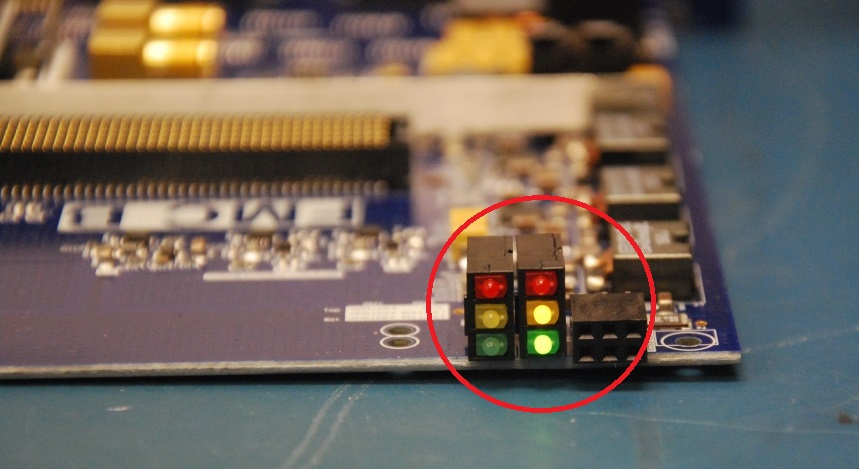
\includegraphics[width=0.7\linewidth]{./IceBoardPhotos/PLLTest/PLLLock.jpeg}
	\caption{PLL Lock LEDs}
	\label{fig:PLLLights}
\end{figure}

\pagebreak
\subsection{Memory test}

\textbf{Step 1}: Insert a valid SD card into the front slot - see figure \ref{fig:MemSDCard}.
\begin{figure}[!htbp]
	\centering
	\includegraphics[width=0.7\linewidth]{./IceBoardPhotos/MemTest/SD_card.jpeg}
	\caption{SD Card plugged into the motherboard}
	\label{fig:MemSDCard}
\end{figure}

\noindent \textbf{Step 2}: Connect the RS232 dongle to the bottom pins on the front of the board, and then the other end into a USB port of the test computer - see figure \ref{fig:MemRS232}.

\begin{figure}[!htbp]
	\centering
	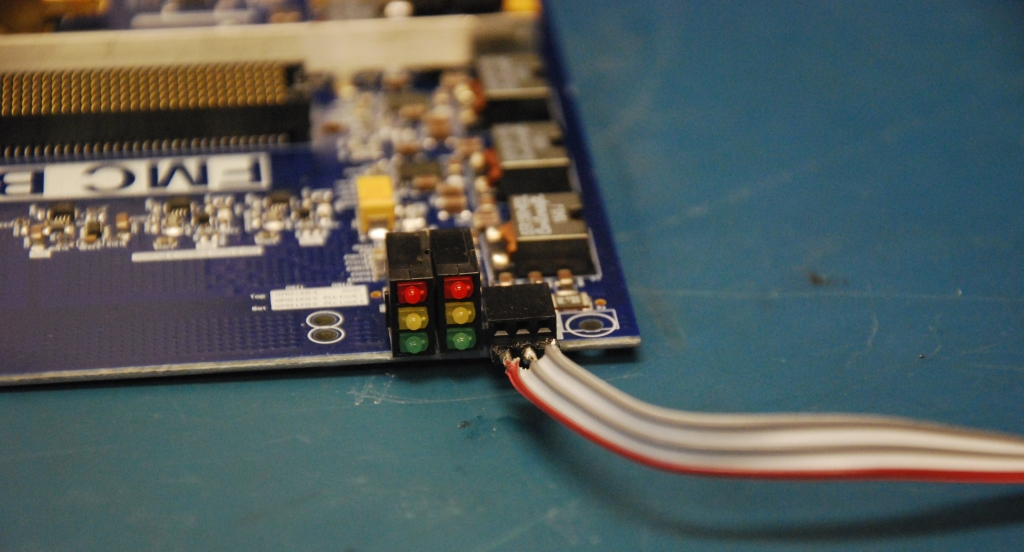
\includegraphics[width=0.7\linewidth]{./IceBoardPhotos/MemTest/RS232_dongle.jpeg}
	\caption{RS232 dongle attached to motherboard}
	\label{fig:MemRS232}
\end{figure}

\pagebreak
\subsection{Tests that require networking}

For all ensuing tests (Serial number programming, Clock testing, I2C device testing, Power sensor readout, FPGA programming, QSFP testing, GTX link quality testing, Mezzanine testing, Ramp testing), make sure you have an Ethernet cable plugged into the second port from the edge as shown in - see figure \ref{fig:NetSetupEth}.

\begin{figure}[!htbp]
	\centering
	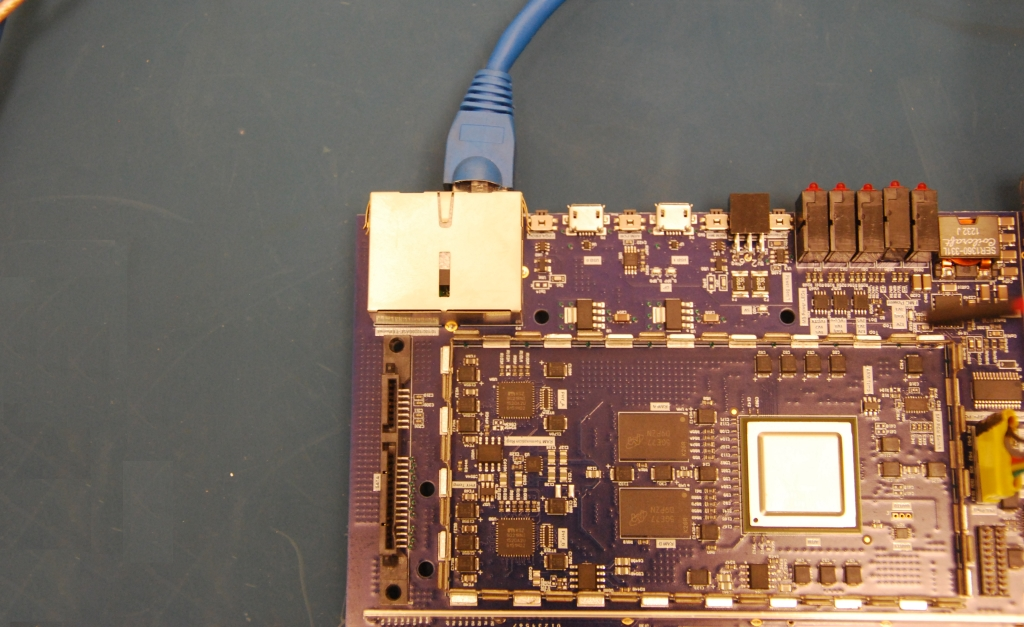
\includegraphics[width=0.7\linewidth]{./IceBoardPhotos/NetTest/ethernet.jpeg}
	\caption{Ethernet cable attached to ARM processor}
	\label{fig:NetSetupEth}
\end{figure}

\noindent Make sure that a valid SD card is present in the front slot - see figure \ref{fig:NetSetupSD}.

\begin{figure}[!htbp]
	\centering
	\includegraphics[width=0.7\linewidth]{./IceBoardPhotos/NetTest/SD_card.jpeg}
	\caption{SD Card plugged into the motherboard}
	\label{fig:NetSetupSD}
\end{figure}


\subsection{Serial number programming}
No additional setup/steps are required for this test

\subsection{Clock testing}

\textbf{Warning} : It is good practice in this test to terminate the SMA clock jumper cable when the cable is not in use. This termination however is only critical when performing Step 3. 
\newline

\noindent\textbf{Step 1}: Testing the onboard crystal. Set the jumper into the crystal position (left) as shown in the figure \ref{fig:ClockCrystal}.

\begin{figure}[!htbp]
	\centering
	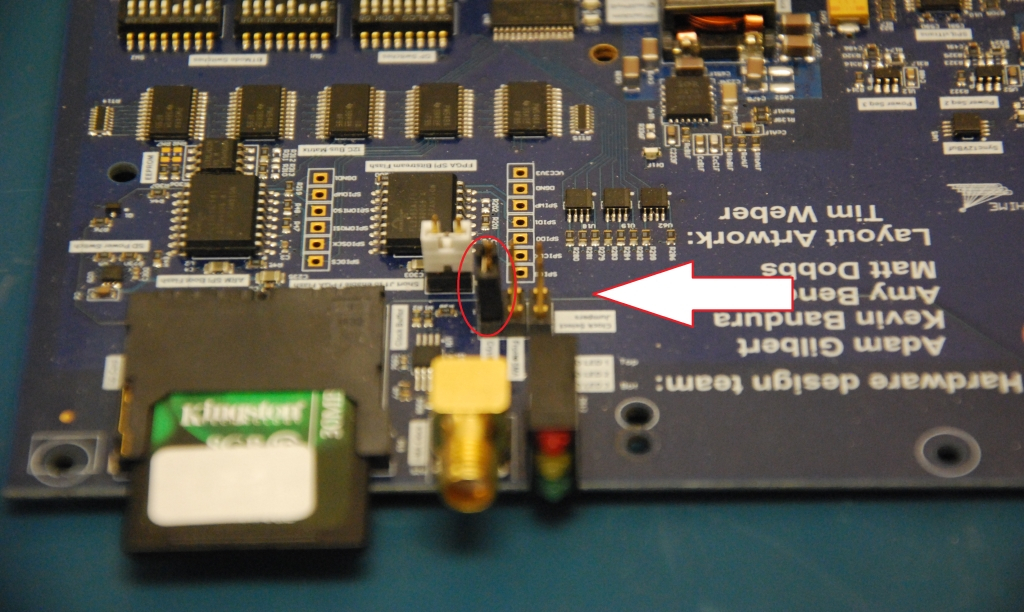
\includegraphics[width=0.8\linewidth]{./IceBoardPhotos/ClockTest/clock_jumper.jpeg}
	\caption{Clock select jumper in onboard crystal position}
	\label{fig:ClockCrystal}
\end{figure}

\noindent\textbf{Step 2}: Testing the front panel SMA clock input. Set the jumper into the front SMA position (middle), and connect the SMA to the front panel SMA connector - as shown in the figure \ref{fig:ClockSMA}. Make sure that the other end of the SMA cable is connected to the backplane as shown in figure \ref{fig:ClockBackplaneSMA}
\newline

\noindent\textbf{Step 3} : Testing the backplane clock. Set the jumper back to its original position (right). Make sure that the front panel SMA clock cable is terminated.

\begin{figure}[!htbp]
	\centering
	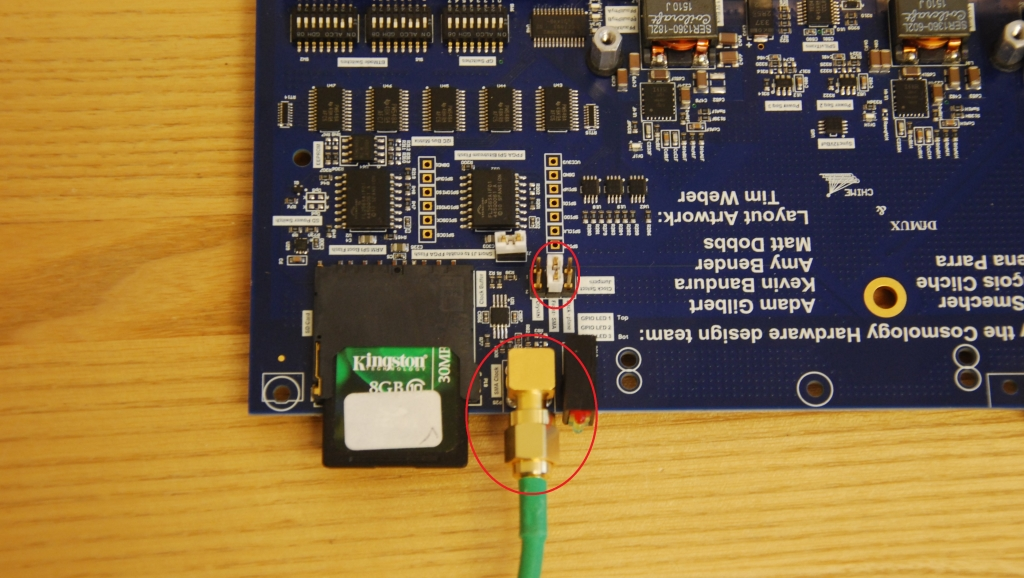
\includegraphics[width=\linewidth]{./IceBoardPhotos/ClockTest/front_sma.jpeg}
	\caption{Clock select jumper in Front panel SMA mode - Clocking cable attached to the board}
	\label{fig:ClockSMA}
\end{figure}

\begin{figure}[!htbp]
	\centering
	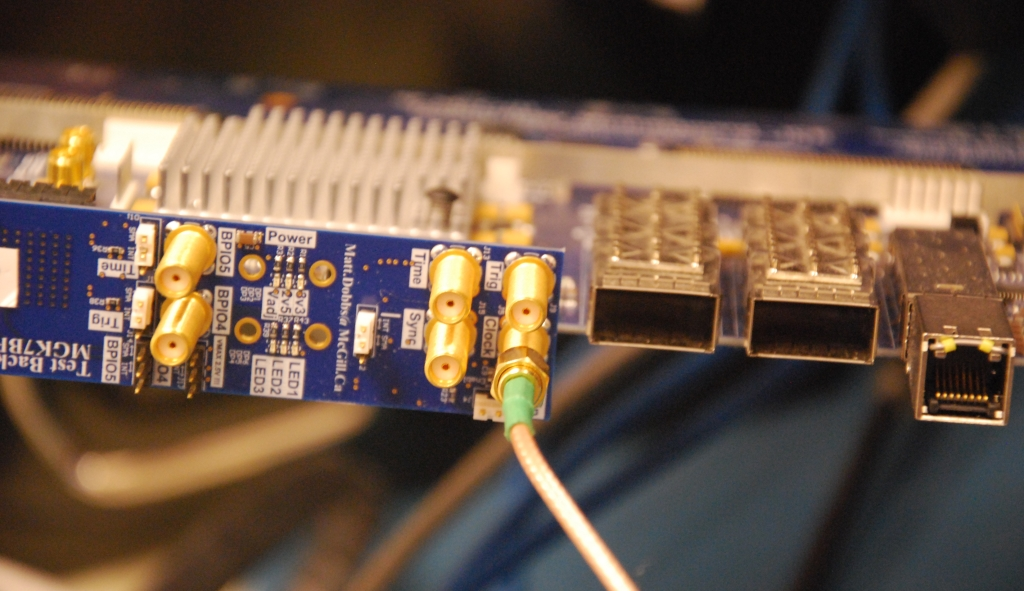
\includegraphics[width=\linewidth]{./IceBoardPhotos/ClockTest/backplane_clock.jpeg}
	\caption{Clocking cable attached to backplane}
	\label{fig:ClockBackplaneSMA}
\end{figure}

\pagebreak

\subsection{I2C}
No additional setup/steps are required for this test.

\subsection{Sensors}
No additional setup/steps are required for this test. Ensure that the mezzanines are not loaded.

\subsection{FPGA Test - and all ensuing tests}

This setup will be required for the QSFP test, GTX link testing, basic Mezzanine test, and Ramp test.

Note that if you complete the hardware setups for all other tests. In the test suite you can request that the tests run in order until a failure occurs e.g 10-14. This can save significant time since most boards will pass this step and it takes about 15 minutes to complete these 5 tests.

\medskip\noindent\textbf{Step 1}: Ensure that an SFP adapter is plugged into the motherboard and connect an Ethernet cable into the adapter - as shown in figure \ref{fig:FPGASetup}

\begin{figure}[!htbp]
	\centering
	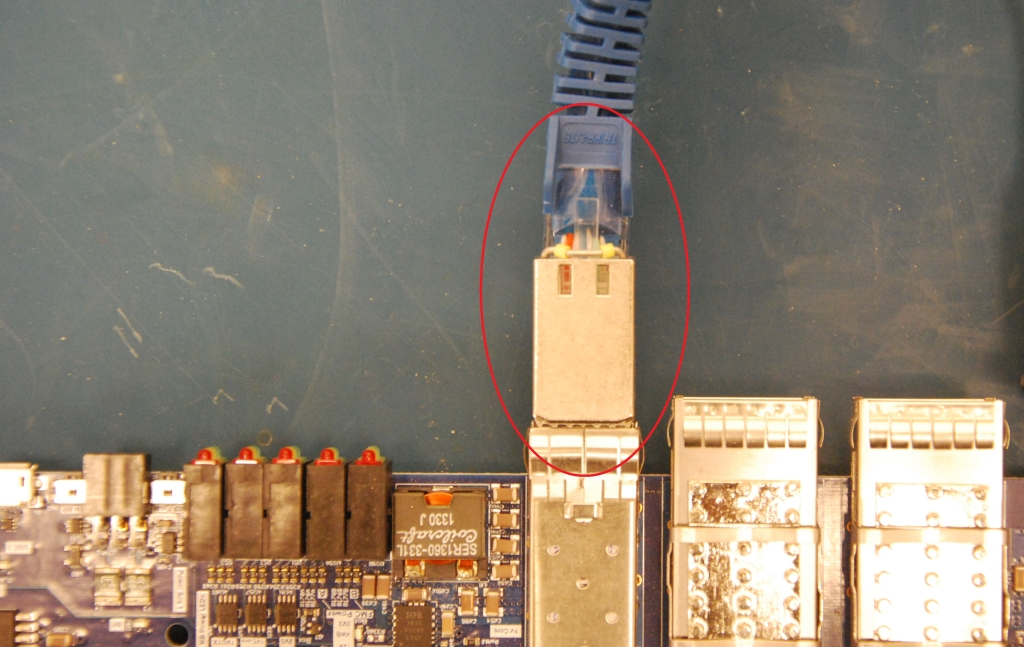
\includegraphics[width=\linewidth]{./IceBoardPhotos/FPGATest/fpga_ethernet.jpeg}
	\caption{Ethernet cable, and SFP adapter plugged into the motherboard}
	\label{fig:FPGASetup}
\end{figure}

\medskip\noindent\textbf{Step 2}: Mount the FPGA fan to the heatsink and attach the cable as shown in figure \ref{fig:FPGAfan}

\begin{figure}[!htbp]
	\centering
	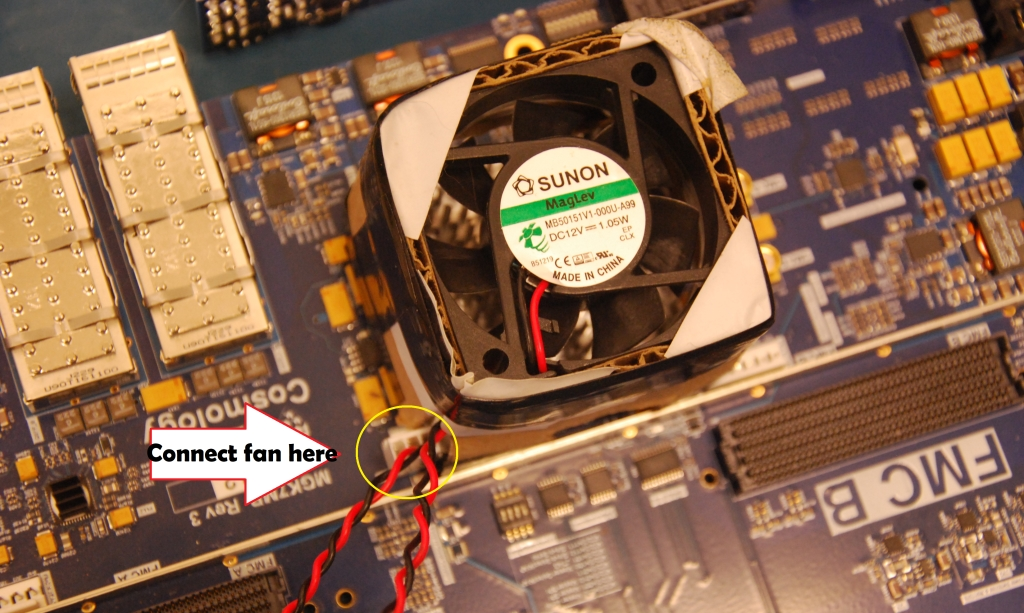
\includegraphics[width=\linewidth]{./IceBoardPhotos/FPGATest/fpga_fan.jpeg}
	\caption{Fan to cool the FPGA mounted onto the motherboard}
	\label{fig:FPGAfan}
\end{figure}

\pagebreak
\subsection{QSFP test}
Make sure that the FPGA test setup - has been completed to start this test.

\medskip
\noindent\textbf{Step 1}: Connect the QSFP cable in a loopback configuration as shown in figure \ref{fig:QSFPloop}. This setup is also required for the GTX test.

\begin{figure}[!htbp]
	\centering
	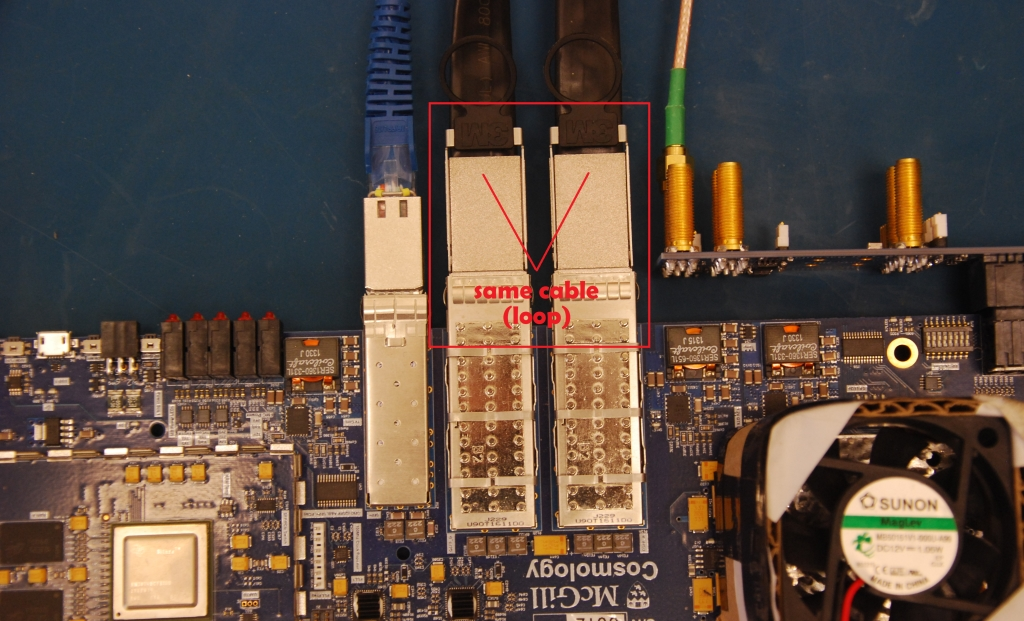
\includegraphics[width=\linewidth]{./IceBoardPhotos/QSFPTest/qsfp_loop.jpeg}
	\caption{QSFP Cable in a loop back configuration}
	\label{fig:QSFPloop}
\end{figure}

\pagebreak
\subsection{GTX test}
Make sure that the FPGA test setup, as well as QSFP test setup have been completed to start this test. Mezzanines can be loaded (makes no difference).


\subsection{Mezzanine test}
Mount both mezzanines onto the motherboard. Please use the extender cables to protect the mezzanine connectors from repeated insertions.

\subsection{Ramp test}
Mount both mezzanines onto the motherboard. Please use the extender cables to protect the mezzanine connectors from repeated insertions.
















